\documentclass[twoside]{book}

% Packages required by doxygen
\usepackage{fixltx2e}
\usepackage{calc}
\usepackage{doxygen}
\usepackage{graphicx}
\usepackage[utf8]{inputenc}
\usepackage{makeidx}
\usepackage{multicol}
\usepackage{multirow}
\PassOptionsToPackage{warn}{textcomp}
\usepackage{textcomp}
\usepackage[nointegrals]{wasysym}
\usepackage[table]{xcolor}

% NLS support packages
\usepackage[french]{babel}

% Font selection
\usepackage[T1]{fontenc}
\usepackage{mathptmx}
\usepackage[scaled=.90]{helvet}
\usepackage{courier}
\usepackage{amssymb}
\usepackage{sectsty}
\renewcommand{\familydefault}{\sfdefault}
\allsectionsfont{%
  \fontseries{bc}\selectfont%
  \color{darkgray}%
}
\renewcommand{\DoxyLabelFont}{%
  \fontseries{bc}\selectfont%
  \color{darkgray}%
}
\newcommand{\+}{\discretionary{\mbox{\scriptsize$\hookleftarrow$}}{}{}}

% Page & text layout
\usepackage{geometry}
\geometry{%
  a4paper,%
  top=2.5cm,%
  bottom=2.5cm,%
  left=2.5cm,%
  right=2.5cm%
}
\tolerance=750
\hfuzz=15pt
\hbadness=750
\setlength{\emergencystretch}{15pt}
\setlength{\parindent}{0cm}
\setlength{\parskip}{0.2cm}
\makeatletter
\renewcommand{\paragraph}{%
  \@startsection{paragraph}{4}{0ex}{-1.0ex}{1.0ex}{%
    \normalfont\normalsize\bfseries\SS@parafont%
  }%
}
\renewcommand{\subparagraph}{%
  \@startsection{subparagraph}{5}{0ex}{-1.0ex}{1.0ex}{%
    \normalfont\normalsize\bfseries\SS@subparafont%
  }%
}
\makeatother

% Headers & footers
\usepackage{fancyhdr}
\pagestyle{fancyplain}
\fancyhead[LE]{\fancyplain{}{\bfseries\thepage}}
\fancyhead[CE]{\fancyplain{}{}}
\fancyhead[RE]{\fancyplain{}{\bfseries\leftmark}}
\fancyhead[LO]{\fancyplain{}{\bfseries\rightmark}}
\fancyhead[CO]{\fancyplain{}{}}
\fancyhead[RO]{\fancyplain{}{\bfseries\thepage}}
\fancyfoot[LE]{\fancyplain{}{}}
\fancyfoot[CE]{\fancyplain{}{}}
\fancyfoot[RE]{\fancyplain{}{\bfseries\scriptsize Généré le Vendredi 20 Mars 2015 11\+:07\+:21 pour C\+R\+T\+C par Doxygen }}
\fancyfoot[LO]{\fancyplain{}{\bfseries\scriptsize Généré le Vendredi 20 Mars 2015 11\+:07\+:21 pour C\+R\+T\+C par Doxygen }}
\fancyfoot[CO]{\fancyplain{}{}}
\fancyfoot[RO]{\fancyplain{}{}}
\renewcommand{\footrulewidth}{0.4pt}
\renewcommand{\chaptermark}[1]{%
  \markboth{#1}{}%
}
\renewcommand{\sectionmark}[1]{%
  \markright{\thesection\ #1}%
}

% Indices & bibliography
\usepackage{natbib}
\usepackage[titles]{tocloft}
\setcounter{tocdepth}{3}
\setcounter{secnumdepth}{5}
\makeindex

% Hyperlinks (required, but should be loaded last)
\usepackage{ifpdf}
\ifpdf
  \usepackage[pdftex,pagebackref=true]{hyperref}
\else
  \usepackage[ps2pdf,pagebackref=true]{hyperref}
\fi
\hypersetup{%
  colorlinks=true,%
  linkcolor=blue,%
  citecolor=blue,%
  unicode%
}

% Custom commands
\newcommand{\clearemptydoublepage}{%
  \newpage{\pagestyle{empty}\cleardoublepage}%
}


%===== C O N T E N T S =====

\begin{document}

% Titlepage & ToC
\hypersetup{pageanchor=false,
             bookmarks=true,
             bookmarksnumbered=true,
             pdfencoding=unicode
            }
\pagenumbering{roman}
\begin{titlepage}
\vspace*{7cm}
\begin{center}%
{\Large C\+R\+T\+C }\\
\vspace*{1cm}
{\large Généré par Doxygen 1.8.8}\\
\vspace*{0.5cm}
{\small Vendredi 20 Mars 2015 11:07:21}\\
\end{center}
\end{titlepage}
\clearemptydoublepage
\tableofcontents
\clearemptydoublepage
\pagenumbering{arabic}
\hypersetup{pageanchor=true}

%--- Begin generated contents ---
\chapter{Classe C\+I2\+C}
\label{index}\hypertarget{index}{}\begin{DoxyAuthor}{Auteur}
Simon Moinet 
\end{DoxyAuthor}
\begin{DoxyDate}{Date}
Mars 2015
\end{DoxyDate}
Cette classe \hyperlink{classCI2C}{C\+I2\+C} permet de lire/écrire les valeurs de registres des esclaves d'un bus I2\+C 
\chapter{Index hiérarchique}
\section{Hiérarchie des classes}
Cette liste d'héritage est classée approximativement par ordre alphabétique \+:\begin{DoxyCompactList}
\item \contentsline{section}{C\+I2\+C}{\pageref{classCI2C}}{}
\begin{DoxyCompactList}
\item \contentsline{section}{C\+R\+T\+C}{\pageref{classCRTC}}{}
\end{DoxyCompactList}
\item std\+:\+:exception\begin{DoxyCompactList}
\item \contentsline{section}{C\+I2\+C\+:\+:Erreur\+Dev\+Not\+Define}{\pageref{classCI2C_1_1ErreurDevNotDefine}}{}
\item \contentsline{section}{C\+I2\+C\+:\+:Erreur\+Open\+Dev}{\pageref{classCI2C_1_1ErreurOpenDev}}{}
\item \contentsline{section}{C\+I2\+C\+:\+:Erreur\+Read}{\pageref{classCI2C_1_1ErreurRead}}{}
\item \contentsline{section}{C\+I2\+C\+:\+:Erreur\+Set\+Addr\+Slave}{\pageref{classCI2C_1_1ErreurSetAddrSlave}}{}
\item \contentsline{section}{C\+I2\+C\+:\+:Erreur\+Slave\+Not\+Define}{\pageref{classCI2C_1_1ErreurSlaveNotDefine}}{}
\item \contentsline{section}{C\+I2\+C\+:\+:Erreur\+Write}{\pageref{classCI2C_1_1ErreurWrite}}{}
\end{DoxyCompactList}
\end{DoxyCompactList}

\chapter{Index des classes}
\section{Liste des classes}
Liste des classes, structures, unions et interfaces avec une brève description \+:\begin{DoxyCompactList}
\item\contentsline{section}{\hyperlink{classCI2C}{C\+I2\+C} \\*Cette classe \hyperlink{classCI2C}{C\+I2\+C} permet de lire/écrire les valeurs de registres des esclaves d'un bus I2\+C }{\pageref{classCI2C}}{}
\item\contentsline{section}{\hyperlink{classCRTC}{C\+R\+T\+C} \\*Cette classe permet }{\pageref{classCRTC}}{}
\item\contentsline{section}{\hyperlink{classCI2C_1_1ErreurDevNotDefine}{C\+I2\+C\+::\+Erreur\+Dev\+Not\+Define} }{\pageref{classCI2C_1_1ErreurDevNotDefine}}{}
\item\contentsline{section}{\hyperlink{classCI2C_1_1ErreurOpenDev}{C\+I2\+C\+::\+Erreur\+Open\+Dev} }{\pageref{classCI2C_1_1ErreurOpenDev}}{}
\item\contentsline{section}{\hyperlink{classCI2C_1_1ErreurRead}{C\+I2\+C\+::\+Erreur\+Read} }{\pageref{classCI2C_1_1ErreurRead}}{}
\item\contentsline{section}{\hyperlink{classCI2C_1_1ErreurSetAddrSlave}{C\+I2\+C\+::\+Erreur\+Set\+Addr\+Slave} }{\pageref{classCI2C_1_1ErreurSetAddrSlave}}{}
\item\contentsline{section}{\hyperlink{classCI2C_1_1ErreurSlaveNotDefine}{C\+I2\+C\+::\+Erreur\+Slave\+Not\+Define} }{\pageref{classCI2C_1_1ErreurSlaveNotDefine}}{}
\item\contentsline{section}{\hyperlink{classCI2C_1_1ErreurWrite}{C\+I2\+C\+::\+Erreur\+Write} }{\pageref{classCI2C_1_1ErreurWrite}}{}
\end{DoxyCompactList}

\chapter{Index des fichiers}
\section{Liste des fichiers}
Liste de tous les fichiers documentés avec une brève description \+:\begin{DoxyCompactList}
\item\contentsline{section}{/home/jam/\+Bureau/\+C++/\+Classes/\+C\+R\+T\+C/\hyperlink{CRTC_8h}{C\+R\+T\+C.\+h} }{\pageref{CRTC_8h}}{}
\item\contentsline{section}{/home/jam/\+Bureau/\+C++/\+Classes/\+C\+R\+T\+C/\+C\+I2\+C/\hyperlink{CI2C_8cpp}{C\+I2\+C.\+cpp} \\*Contient la définition de la classe \hyperlink{classCI2C}{C\+I2\+C} }{\pageref{CI2C_8cpp}}{}
\item\contentsline{section}{/home/jam/\+Bureau/\+C++/\+Classes/\+C\+R\+T\+C/\+C\+I2\+C/\hyperlink{CI2C_8h}{C\+I2\+C.\+h} \\*Contient la declaration de la \hyperlink{classCI2C}{C\+I2\+C} }{\pageref{CI2C_8h}}{}
\end{DoxyCompactList}

\chapter{Documentation des classes}
\hypertarget{classCI2C}{\section{Référence de la classe C\+I2\+C}
\label{classCI2C}\index{C\+I2\+C@{C\+I2\+C}}
}


Cette classe \hyperlink{classCI2C}{C\+I2\+C} permet de lire/écrire les valeurs de registres des esclaves d'un bus I2\+C.  




{\ttfamily \#include $<$C\+I2\+C.\+h$>$}



Graphe d'héritage de C\+I2\+C\+:
\nopagebreak
\begin{figure}[H]
\begin{center}
\leavevmode
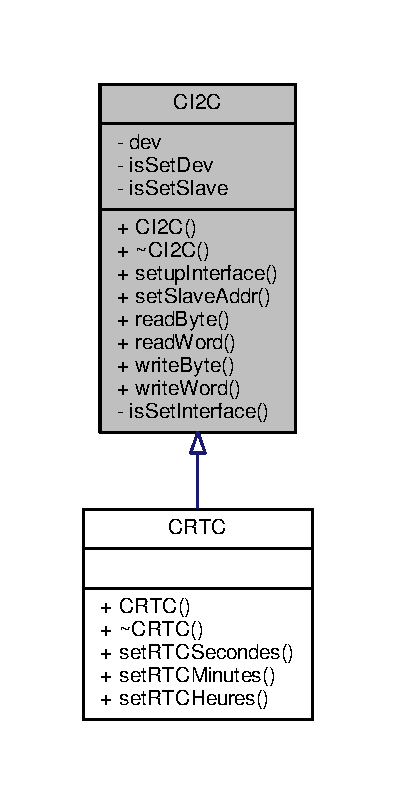
\includegraphics[width=190pt]{classCI2C__inherit__graph}
\end{center}
\end{figure}


Graphe de collaboration de C\+I2\+C\+:
\nopagebreak
\begin{figure}[H]
\begin{center}
\leavevmode
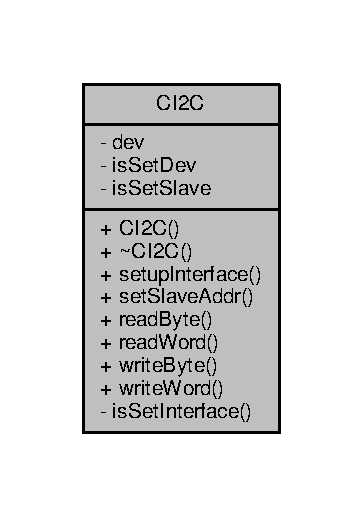
\includegraphics[width=174pt]{classCI2C__coll__graph}
\end{center}
\end{figure}
\subsection*{Classes}
\begin{DoxyCompactItemize}
\item 
class \hyperlink{classCI2C_1_1ErreurDevNotDefine}{Erreur\+Dev\+Not\+Define}
\item 
class \hyperlink{classCI2C_1_1ErreurOpenDev}{Erreur\+Open\+Dev}
\item 
class \hyperlink{classCI2C_1_1ErreurRead}{Erreur\+Read}
\item 
class \hyperlink{classCI2C_1_1ErreurSetAddrSlave}{Erreur\+Set\+Addr\+Slave}
\item 
class \hyperlink{classCI2C_1_1ErreurSlaveNotDefine}{Erreur\+Slave\+Not\+Define}
\item 
class \hyperlink{classCI2C_1_1ErreurWrite}{Erreur\+Write}
\end{DoxyCompactItemize}
\subsection*{Fonctions membres publiques}
\begin{DoxyCompactItemize}
\item 
\hyperlink{classCI2C_a2df83a2627a8b8bf91460a68372c9ed5}{C\+I2\+C} ()
\begin{DoxyCompactList}\small\item\em Constructeur de la classe \hyperlink{classCI2C}{C\+I2\+C}. \end{DoxyCompactList}\item 
\hypertarget{classCI2C_ae757710bb84ab327217092f0af851a16}{\hyperlink{classCI2C_ae757710bb84ab327217092f0af851a16}{$\sim$\+C\+I2\+C} ()}\label{classCI2C_ae757710bb84ab327217092f0af851a16}

\begin{DoxyCompactList}\small\item\em Destructeur de la classe \hyperlink{classCI2C}{C\+I2\+C}. \end{DoxyCompactList}\item 
void \hyperlink{classCI2C_a8fe8755470906582ab854edcbf2a2992}{setup\+Interface} (string \hyperlink{classCI2C_ae2d4648eadc2acae86a49cecbf39ce56}{dev}, \+\_\+\+\_\+u8 addr\+\_\+slave)
\begin{DoxyCompactList}\small\item\em Methode setup\+Interface. \end{DoxyCompactList}\item 
void \hyperlink{classCI2C_ae766fc56ba88f9063e86412fca0c1dfc}{set\+Slave\+Addr} (\+\_\+\+\_\+u8 addr\+\_\+slave)
\begin{DoxyCompactList}\small\item\em Methode set\+Slave\+Addr. \end{DoxyCompactList}\item 
int \hyperlink{classCI2C_afb589b9bdefa75257807b4e6ac2c1c5a}{read\+Byte} (\+\_\+\+\_\+u8 reg=0)
\begin{DoxyCompactList}\small\item\em Methode read\+Byte. \end{DoxyCompactList}\item 
int \hyperlink{classCI2C_a283d5f6d8371e2abb6532b9e32392f9a}{read\+Word} (\+\_\+\+\_\+u8 reg=0)
\begin{DoxyCompactList}\small\item\em Methode read\+Word. \end{DoxyCompactList}\item 
void \hyperlink{classCI2C_a26517fc7e3a282863ff09e7a792f4386}{write\+Byte} (\+\_\+\+\_\+u8 reg, \+\_\+\+\_\+u8 data)
\begin{DoxyCompactList}\small\item\em Methode write\+Byte. \end{DoxyCompactList}\item 
void \hyperlink{classCI2C_a14250174d9281db1bc1db2360cacee40}{write\+Word} (\+\_\+\+\_\+u8 reg, \+\_\+\+\_\+u16 data)
\begin{DoxyCompactList}\small\item\em Methode write\+Word. \end{DoxyCompactList}\end{DoxyCompactItemize}
\subsection*{Fonctions membres privées}
\begin{DoxyCompactItemize}
\item 
void \hyperlink{classCI2C_a821adb4a309a1377fef4d1b8487a731e}{is\+Set\+Interface} ()
\begin{DoxyCompactList}\small\item\em Methode is\+Set\+Interface. \end{DoxyCompactList}\end{DoxyCompactItemize}
\subsection*{Attributs privés}
\begin{DoxyCompactItemize}
\item 
\hypertarget{classCI2C_ae2d4648eadc2acae86a49cecbf39ce56}{int \hyperlink{classCI2C_ae2d4648eadc2acae86a49cecbf39ce56}{dev}}\label{classCI2C_ae2d4648eadc2acae86a49cecbf39ce56}

\begin{DoxyCompactList}\small\item\em Contient les informations du bus I2\+C. \end{DoxyCompactList}\item 
\hypertarget{classCI2C_a892d111f995589334497f2b573ab436d}{bool \hyperlink{classCI2C_a892d111f995589334497f2b573ab436d}{is\+Set\+Dev}}\label{classCI2C_a892d111f995589334497f2b573ab436d}

\begin{DoxyCompactList}\small\item\em Bool qui permet de savoir si le dev est défini. \end{DoxyCompactList}\item 
\hypertarget{classCI2C_a19200c12efe17b560256641cce4f5909}{bool \hyperlink{classCI2C_a19200c12efe17b560256641cce4f5909}{is\+Set\+Slave}}\label{classCI2C_a19200c12efe17b560256641cce4f5909}

\begin{DoxyCompactList}\small\item\em Bool qui permet de savoir sur l'esclave est défini. \end{DoxyCompactList}\end{DoxyCompactItemize}


\subsection{Description détaillée}
Cette classe \hyperlink{classCI2C}{C\+I2\+C} permet de lire/écrire les valeurs de registres des esclaves d'un bus I2\+C. 

\subsection{Documentation des constructeurs et destructeur}
\hypertarget{classCI2C_a2df83a2627a8b8bf91460a68372c9ed5}{\index{C\+I2\+C@{C\+I2\+C}!C\+I2\+C@{C\+I2\+C}}
\index{C\+I2\+C@{C\+I2\+C}!C\+I2\+C@{C\+I2\+C}}
\subsubsection[{C\+I2\+C}]{\setlength{\rightskip}{0pt plus 5cm}C\+I2\+C\+::\+C\+I2\+C (
\begin{DoxyParamCaption}
{}
\end{DoxyParamCaption}
)}}\label{classCI2C_a2df83a2627a8b8bf91460a68372c9ed5}


Constructeur de la classe \hyperlink{classCI2C}{C\+I2\+C}. 

Ce constructeur initialise les attributs de la classe. 

Références dev, is\+Set\+Dev, et is\+Set\+Slave.



\subsection{Documentation des fonctions membres}
\hypertarget{classCI2C_a821adb4a309a1377fef4d1b8487a731e}{\index{C\+I2\+C@{C\+I2\+C}!is\+Set\+Interface@{is\+Set\+Interface}}
\index{is\+Set\+Interface@{is\+Set\+Interface}!C\+I2\+C@{C\+I2\+C}}
\subsubsection[{is\+Set\+Interface}]{\setlength{\rightskip}{0pt plus 5cm}void C\+I2\+C\+::is\+Set\+Interface (
\begin{DoxyParamCaption}
{}
\end{DoxyParamCaption}
)\hspace{0.3cm}{\ttfamily [private]}}}\label{classCI2C_a821adb4a309a1377fef4d1b8487a731e}


Methode is\+Set\+Interface. 

Cette méthode permet de verifier si le dev et l'esclave sont bien défini


\begin{DoxyExceptions}{Exceptions}
{\em String\+Index\+Out\+Of\+Range\+Exception} & if index is not between {\ttfamily 0} and {\ttfamily length() -\/ 1}. \\
\hline
{\em Erreur(\+T\+Y\+P\+E\+\_\+\+E\+R\+R\+E\+U\+R} & erreur, string const\& phrase) Si le dev n'est pas défini, leve une exception de type Erreur\+::\+T\+Y\+P\+E\+\_\+\+E\+R\+R\+E\+U\+R\+::\+D\+E\+V\+\_\+\+D\+E\+F \\
\hline
{\em Erreur(\+T\+Y\+P\+E\+\_\+\+E\+R\+R\+E\+U\+R} & erreur, string const\& phrase) Si l'esclave n'est pas défini, leve une exception de type Erreur\+::\+T\+Y\+P\+E\+\_\+\+E\+R\+R\+E\+U\+R\+::\+S\+L\+A\+V\+E\+\_\+\+D\+E\+F \\
\hline
\end{DoxyExceptions}


Références is\+Set\+Dev, et is\+Set\+Slave.



Référencé par read\+Byte(), read\+Word(), write\+Byte(), et write\+Word().

\hypertarget{classCI2C_afb589b9bdefa75257807b4e6ac2c1c5a}{\index{C\+I2\+C@{C\+I2\+C}!read\+Byte@{read\+Byte}}
\index{read\+Byte@{read\+Byte}!C\+I2\+C@{C\+I2\+C}}
\subsubsection[{read\+Byte}]{\setlength{\rightskip}{0pt plus 5cm}int C\+I2\+C\+::read\+Byte (
\begin{DoxyParamCaption}
\item[{\+\_\+\+\_\+u8}]{reg = {\ttfamily 0}}
\end{DoxyParamCaption}
)}}\label{classCI2C_afb589b9bdefa75257807b4e6ac2c1c5a}


Methode read\+Byte. 

Lecture du registre sur un octet. Par default la valeur est fixé à zéro dans le cas d'un esclave sans registre


\begin{DoxyParams}[1]{Paramètres}
\mbox{\tt in}  & {\em reg} & \+: le registre que l'on veux lire \\
\hline
\end{DoxyParams}
\begin{DoxyReturn}{Renvoie}
Un int contenant l'octet du registre lu 
\end{DoxyReturn}


Références dev, et is\+Set\+Interface().

\hypertarget{classCI2C_a283d5f6d8371e2abb6532b9e32392f9a}{\index{C\+I2\+C@{C\+I2\+C}!read\+Word@{read\+Word}}
\index{read\+Word@{read\+Word}!C\+I2\+C@{C\+I2\+C}}
\subsubsection[{read\+Word}]{\setlength{\rightskip}{0pt plus 5cm}int C\+I2\+C\+::read\+Word (
\begin{DoxyParamCaption}
\item[{\+\_\+\+\_\+u8}]{reg = {\ttfamily 0}}
\end{DoxyParamCaption}
)}}\label{classCI2C_a283d5f6d8371e2abb6532b9e32392f9a}


Methode read\+Word. 

Lecture du registre sur deux octets. Par default la valeur est ficé à zéro dans le cas d'un esclave sans registre


\begin{DoxyParams}[1]{Paramètres}
\mbox{\tt in}  & {\em reg} & \+: le registre que l'on veux lire \\
\hline
\end{DoxyParams}
\begin{DoxyReturn}{Renvoie}
Un int contenant les deux octets du registre lu 
\end{DoxyReturn}


Références dev, et is\+Set\+Interface().

\hypertarget{classCI2C_ae766fc56ba88f9063e86412fca0c1dfc}{\index{C\+I2\+C@{C\+I2\+C}!set\+Slave\+Addr@{set\+Slave\+Addr}}
\index{set\+Slave\+Addr@{set\+Slave\+Addr}!C\+I2\+C@{C\+I2\+C}}
\subsubsection[{set\+Slave\+Addr}]{\setlength{\rightskip}{0pt plus 5cm}void C\+I2\+C\+::set\+Slave\+Addr (
\begin{DoxyParamCaption}
\item[{\+\_\+\+\_\+u8}]{addr\+\_\+slave}
\end{DoxyParamCaption}
)}}\label{classCI2C_ae766fc56ba88f9063e86412fca0c1dfc}


Methode set\+Slave\+Addr. 

Paramétrage de la nouvelle addresse de l'esclave sur le bus I2\+C


\begin{DoxyParams}[1]{Paramètres}
\mbox{\tt in}  & {\em \+\_\+\+\_\+u8} & addr\+\_\+slave \+: la nouvelle addresse de l'esclave\\
\hline
\end{DoxyParams}

\begin{DoxyExceptions}{Exceptions}
{\em Erreur(\+T\+Y\+P\+E\+\_\+\+E\+R\+R\+E\+U\+R} & erreur, string const\& phrase) Si le dev n'est pas défini, leve une exception de type Erreur\+::\+T\+Y\+P\+E\+\_\+\+E\+R\+R\+E\+U\+R\+::\+D\+E\+V\+\_\+\+D\+E\+F \\
\hline
{\em Erreur(\+T\+Y\+P\+E\+\_\+\+E\+R\+R\+E\+U\+R} & erreur, string const\& phrase) Si la spécification de l'adresse de l'esclave avec lequel on veux communiquer à échoué. Leve une exception de type Erreur\+::\+T\+Y\+P\+E\+\_\+\+E\+R\+R\+E\+U\+R\+::\+S\+L\+A\+V\+E\+\_\+\+D\+E\+F \\
\hline
\end{DoxyExceptions}


Références dev, is\+Set\+Dev, et is\+Set\+Slave.

\hypertarget{classCI2C_a8fe8755470906582ab854edcbf2a2992}{\index{C\+I2\+C@{C\+I2\+C}!setup\+Interface@{setup\+Interface}}
\index{setup\+Interface@{setup\+Interface}!C\+I2\+C@{C\+I2\+C}}
\subsubsection[{setup\+Interface}]{\setlength{\rightskip}{0pt plus 5cm}void C\+I2\+C\+::setup\+Interface (
\begin{DoxyParamCaption}
\item[{string}]{dev, }
\item[{\+\_\+\+\_\+u8}]{addr\+\_\+slave}
\end{DoxyParamCaption}
)}}\label{classCI2C_a8fe8755470906582ab854edcbf2a2992}


Methode setup\+Interface. 

Initialisation de l'interface I2\+C et de son esclave.


\begin{DoxyParams}[1]{Paramètres}
\mbox{\tt in}  & {\em dev} & \+: le nom de l'interface I2\+C \\
\hline
\mbox{\tt in}  & {\em addr\+\_\+slave} & \+: l'addresse de l'esclave sur le bus I2\+C\\
\hline
\end{DoxyParams}

\begin{DoxyExceptions}{Exceptions}
{\em Erreur(\+T\+Y\+P\+E\+\_\+\+E\+R\+R\+E\+U\+R} & erreur, string const\& phrase) Si il est impossible de definir le device du bus I2\+C. Leve une exception de type Erreur\+::\+T\+Y\+P\+E\+\_\+\+E\+R\+R\+E\+U\+R\+::\+D\+E\+V\+\_\+\+D\+E\+F \\
\hline
{\em Erreur(\+T\+Y\+P\+E\+\_\+\+E\+R\+R\+E\+U\+R} & erreur, string const\& phrase) Si la spécification de l'adresse de l'esclave avec lequel on veux communiquer à échoué. Leve une exception de type Erreur\+::\+T\+Y\+P\+E\+\_\+\+E\+R\+R\+E\+U\+R\+::\+S\+L\+A\+V\+E\+\_\+\+D\+E\+F \\
\hline
\end{DoxyExceptions}


Références is\+Set\+Dev, et is\+Set\+Slave.

\hypertarget{classCI2C_a26517fc7e3a282863ff09e7a792f4386}{\index{C\+I2\+C@{C\+I2\+C}!write\+Byte@{write\+Byte}}
\index{write\+Byte@{write\+Byte}!C\+I2\+C@{C\+I2\+C}}
\subsubsection[{write\+Byte}]{\setlength{\rightskip}{0pt plus 5cm}void C\+I2\+C\+::write\+Byte (
\begin{DoxyParamCaption}
\item[{\+\_\+\+\_\+u8}]{reg, }
\item[{\+\_\+\+\_\+u8}]{data}
\end{DoxyParamCaption}
)}}\label{classCI2C_a26517fc7e3a282863ff09e7a792f4386}


Methode write\+Byte. 

Ecriture dans un registre sur un octet


\begin{DoxyParams}[1]{Paramètres}
\mbox{\tt in}  & {\em reg} & \+: le registre où on veux écrire \\
\hline
\mbox{\tt in}  & {\em data} & \+: l'octet que l'on veux ecrire dans le registre \\
\hline
\end{DoxyParams}
\begin{DoxyReturn}{Renvoie}
true si l'écriture a réussi, false sinon 
\end{DoxyReturn}


Références dev, et is\+Set\+Interface().

\hypertarget{classCI2C_a14250174d9281db1bc1db2360cacee40}{\index{C\+I2\+C@{C\+I2\+C}!write\+Word@{write\+Word}}
\index{write\+Word@{write\+Word}!C\+I2\+C@{C\+I2\+C}}
\subsubsection[{write\+Word}]{\setlength{\rightskip}{0pt plus 5cm}void C\+I2\+C\+::write\+Word (
\begin{DoxyParamCaption}
\item[{\+\_\+\+\_\+u8}]{reg, }
\item[{\+\_\+\+\_\+u16}]{data}
\end{DoxyParamCaption}
)}}\label{classCI2C_a14250174d9281db1bc1db2360cacee40}


Methode write\+Word. 

Ecriture dans un registre sur deux octets


\begin{DoxyParams}[1]{Paramètres}
\mbox{\tt in}  & {\em reg} & \+: le registre où on veux écrire \\
\hline
\mbox{\tt in}  & {\em data} & \+: les deux otets que l'on veux ecrire dans le registre \\
\hline
\end{DoxyParams}
\begin{DoxyReturn}{Renvoie}
true si l'écriture a réussi, false sinon 
\end{DoxyReturn}


Références dev, et is\+Set\+Interface().



La documentation de cette classe a été générée à partir des fichiers suivants \+:\begin{DoxyCompactItemize}
\item 
/home/jam/\+Bureau/\+C++/\+Classes/\+C\+R\+T\+C/\+C\+I2\+C/\hyperlink{CI2C_8h}{C\+I2\+C.\+h}\item 
/home/jam/\+Bureau/\+C++/\+Classes/\+C\+R\+T\+C/\+C\+I2\+C/\hyperlink{CI2C_8cpp}{C\+I2\+C.\+cpp}\end{DoxyCompactItemize}

\hypertarget{classCRTC}{\section{Référence de la classe C\+R\+T\+C}
\label{classCRTC}\index{C\+R\+T\+C@{C\+R\+T\+C}}
}


Cette classe permet.  




Graphe d'héritage de C\+R\+T\+C\+:
\nopagebreak
\begin{figure}[H]
\begin{center}
\leavevmode
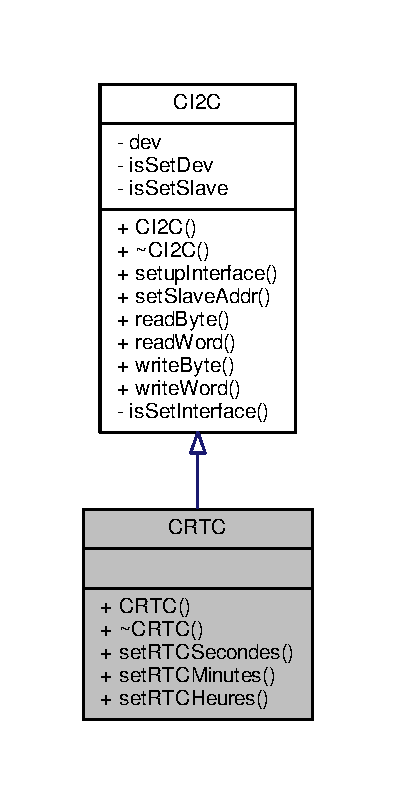
\includegraphics[width=190pt]{classCRTC__inherit__graph}
\end{center}
\end{figure}


Graphe de collaboration de C\+R\+T\+C\+:
\nopagebreak
\begin{figure}[H]
\begin{center}
\leavevmode
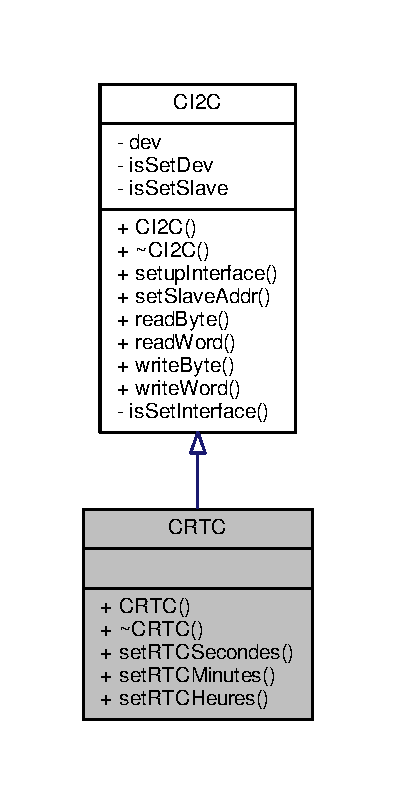
\includegraphics[width=190pt]{classCRTC__coll__graph}
\end{center}
\end{figure}
\subsection*{Types publics}
\begin{DoxyCompactItemize}
\item 
enum \hyperlink{classCRTC_adf700236f14a2071204dc36a75cf4890}{A\+D\+D\+R\+\_\+\+R\+E\+G} \+: \+\_\+\+\_\+u8 \{ \\*
\hyperlink{classCRTC_adf700236f14a2071204dc36a75cf4890af6254ea2451edcc790ea94601f21f927}{A\+D\+D\+R\+\_\+\+R\+E\+G\+::\+S\+E\+C\+O\+N\+D\+E\+S}, 
\hyperlink{classCRTC_adf700236f14a2071204dc36a75cf4890a7ffb9cea885bcba59e55574d54f819c2}{A\+D\+D\+R\+\_\+\+R\+E\+G\+::\+M\+I\+N\+U\+T\+E\+S}, 
\hyperlink{classCRTC_adf700236f14a2071204dc36a75cf4890aca61b64a779fac8c730cfd702fed7a6d}{A\+D\+D\+R\+\_\+\+R\+E\+G\+::\+H\+E\+U\+R\+E\+S}, 
\hyperlink{classCRTC_adf700236f14a2071204dc36a75cf4890a1dd4d26d677c6f4002e7aa611271afcc}{A\+D\+D\+R\+\_\+\+R\+E\+G\+::\+J\+O\+U\+R\+\_\+\+S\+E\+M\+A\+I\+N\+E}, 
\\*
\hyperlink{classCRTC_adf700236f14a2071204dc36a75cf4890a73bbdad552b84783db05ceb17028668b}{A\+D\+D\+R\+\_\+\+R\+E\+G\+::\+J\+O\+U\+R\+\_\+\+M\+O\+I\+S}, 
\hyperlink{classCRTC_adf700236f14a2071204dc36a75cf4890a2256ab3ce73e9b0ee693d8c78cefe7a1}{A\+D\+D\+R\+\_\+\+R\+E\+G\+::\+M\+O\+I\+S}, 
\hyperlink{classCRTC_adf700236f14a2071204dc36a75cf4890a183bf954a3bf4d6fef2515152358aca8}{A\+D\+D\+R\+\_\+\+R\+E\+G\+::\+A\+N\+N\+E\+E}
 \}
\item 
enum \hyperlink{classCRTC_a5b756d38b71f30430a0d4dee80c935a2}{M\+O\+D\+E\+\_\+\+H\+E\+U\+R\+E} \+: \+\_\+\+\_\+u8 \{ \hyperlink{classCRTC_a5b756d38b71f30430a0d4dee80c935a2ac1d9f50f86825a1a2302ec2449c17196}{M\+O\+D\+E\+\_\+\+H\+E\+U\+R\+E\+::\+H}, 
\hyperlink{classCRTC_a5b756d38b71f30430a0d4dee80c935a2ac1d9f50f86825a1a2302ec2449c17196}{M\+O\+D\+E\+\_\+\+H\+E\+U\+R\+E\+::\+H}
 \}
\item 
enum \hyperlink{classCRTC_a7b63c946c21b9e27296d5799c7a96781}{P\+E\+R\+I\+O\+D\+E\+\_\+\+H\+O\+R\+A\+I\+R\+E} \+: \+\_\+\+\_\+u8 \{ \hyperlink{classCRTC_a7b63c946c21b9e27296d5799c7a96781a25ec916d56b8212e569dbf2e4e4b51d4}{P\+E\+R\+I\+O\+D\+E\+\_\+\+H\+O\+R\+A\+I\+R\+E\+::\+A\+M}, 
\hyperlink{classCRTC_a7b63c946c21b9e27296d5799c7a96781a21b7eb30013b04776f5b06bc59209391}{P\+E\+R\+I\+O\+D\+E\+\_\+\+H\+O\+R\+A\+I\+R\+E\+::\+P\+M}
 \}
\end{DoxyCompactItemize}
\subsection*{Fonctions membres publiques}
\begin{DoxyCompactItemize}
\item 
\hypertarget{classCRTC_a33e0a6ea050334a64bc660d8848ce6a0}{\hyperlink{classCRTC_a33e0a6ea050334a64bc660d8848ce6a0}{C\+R\+T\+C} ()}\label{classCRTC_a33e0a6ea050334a64bc660d8848ce6a0}

\begin{DoxyCompactList}\small\item\em Constructeur de la class \hyperlink{classCRTC}{C\+R\+T\+C}. \end{DoxyCompactList}\item 
\hypertarget{classCRTC_a3bb3189c660840a22c45a6a94276a607}{\hyperlink{classCRTC_a3bb3189c660840a22c45a6a94276a607}{$\sim$\+C\+R\+T\+C} ()}\label{classCRTC_a3bb3189c660840a22c45a6a94276a607}

\begin{DoxyCompactList}\small\item\em Destructeur de la classe \hyperlink{classCRTC}{C\+R\+T\+C}. \end{DoxyCompactList}\item 
void \hyperlink{classCRTC_acc2b369b4a007ebbe50097ba647aee61}{set\+R\+T\+C\+Secondes} (int secondes)
\begin{DoxyCompactList}\small\item\em Methode set\+R\+T\+C\+Secondes. \end{DoxyCompactList}\item 
void \hyperlink{classCRTC_af28086ce512a8697c4641f13dba676d8}{set\+R\+T\+C\+Minutes} (int minutes)
\begin{DoxyCompactList}\small\item\em Methode set\+R\+T\+C\+Minutes. \end{DoxyCompactList}\item 
\hypertarget{classCRTC_a3d03c193f47d4950e4727db7d0a96899}{void {\bfseries set\+R\+T\+C\+Heures} (int heures)}\label{classCRTC_a3d03c193f47d4950e4727db7d0a96899}

\end{DoxyCompactItemize}


\subsection{Description détaillée}
Cette classe permet. 

\subsection{Documentation des énumérations membres}
\hypertarget{classCRTC_adf700236f14a2071204dc36a75cf4890}{\index{C\+R\+T\+C@{C\+R\+T\+C}!A\+D\+D\+R\+\_\+\+R\+E\+G@{A\+D\+D\+R\+\_\+\+R\+E\+G}}
\index{A\+D\+D\+R\+\_\+\+R\+E\+G@{A\+D\+D\+R\+\_\+\+R\+E\+G}!C\+R\+T\+C@{C\+R\+T\+C}}
\subsubsection[{A\+D\+D\+R\+\_\+\+R\+E\+G}]{\setlength{\rightskip}{0pt plus 5cm}enum {\bf C\+R\+T\+C\+::\+A\+D\+D\+R\+\_\+\+R\+E\+G} \+: \+\_\+\+\_\+u8\hspace{0.3cm}{\ttfamily [strong]}}}\label{classCRTC_adf700236f14a2071204dc36a75cf4890}
Cette enumeration liste les registres de l'horloge R\+T\+C \begin{Desc}
\item[Valeurs énumérées]\par
\begin{description}
\index{S\+E\+C\+O\+N\+D\+E\+S@{S\+E\+C\+O\+N\+D\+E\+S}!C\+R\+T\+C@{C\+R\+T\+C}}\index{C\+R\+T\+C@{C\+R\+T\+C}!S\+E\+C\+O\+N\+D\+E\+S@{S\+E\+C\+O\+N\+D\+E\+S}}\item[{\em 
\hypertarget{classCRTC_adf700236f14a2071204dc36a75cf4890af6254ea2451edcc790ea94601f21f927}{S\+E\+C\+O\+N\+D\+E\+S}\label{classCRTC_adf700236f14a2071204dc36a75cf4890af6254ea2451edcc790ea94601f21f927}
}]0x01 \+: Registre contenant la valeur des secondes \index{M\+I\+N\+U\+T\+E\+S@{M\+I\+N\+U\+T\+E\+S}!C\+R\+T\+C@{C\+R\+T\+C}}\index{C\+R\+T\+C@{C\+R\+T\+C}!M\+I\+N\+U\+T\+E\+S@{M\+I\+N\+U\+T\+E\+S}}\item[{\em 
\hypertarget{classCRTC_adf700236f14a2071204dc36a75cf4890a7ffb9cea885bcba59e55574d54f819c2}{M\+I\+N\+U\+T\+E\+S}\label{classCRTC_adf700236f14a2071204dc36a75cf4890a7ffb9cea885bcba59e55574d54f819c2}
}]0x01 \+: Registre contenant la valeur des minutes \index{H\+E\+U\+R\+E\+S@{H\+E\+U\+R\+E\+S}!C\+R\+T\+C@{C\+R\+T\+C}}\index{C\+R\+T\+C@{C\+R\+T\+C}!H\+E\+U\+R\+E\+S@{H\+E\+U\+R\+E\+S}}\item[{\em 
\hypertarget{classCRTC_adf700236f14a2071204dc36a75cf4890aca61b64a779fac8c730cfd702fed7a6d}{H\+E\+U\+R\+E\+S}\label{classCRTC_adf700236f14a2071204dc36a75cf4890aca61b64a779fac8c730cfd702fed7a6d}
}]0x02 \+: Registre contenant la valeur des heures \index{J\+O\+U\+R\+\_\+\+S\+E\+M\+A\+I\+N\+E@{J\+O\+U\+R\+\_\+\+S\+E\+M\+A\+I\+N\+E}!C\+R\+T\+C@{C\+R\+T\+C}}\index{C\+R\+T\+C@{C\+R\+T\+C}!J\+O\+U\+R\+\_\+\+S\+E\+M\+A\+I\+N\+E@{J\+O\+U\+R\+\_\+\+S\+E\+M\+A\+I\+N\+E}}\item[{\em 
\hypertarget{classCRTC_adf700236f14a2071204dc36a75cf4890a1dd4d26d677c6f4002e7aa611271afcc}{J\+O\+U\+R\+\_\+\+S\+E\+M\+A\+I\+N\+E}\label{classCRTC_adf700236f14a2071204dc36a75cf4890a1dd4d26d677c6f4002e7aa611271afcc}
}]0x03 \+: Registre contenant le numero du jour de la semaine \index{J\+O\+U\+R\+\_\+\+M\+O\+I\+S@{J\+O\+U\+R\+\_\+\+M\+O\+I\+S}!C\+R\+T\+C@{C\+R\+T\+C}}\index{C\+R\+T\+C@{C\+R\+T\+C}!J\+O\+U\+R\+\_\+\+M\+O\+I\+S@{J\+O\+U\+R\+\_\+\+M\+O\+I\+S}}\item[{\em 
\hypertarget{classCRTC_adf700236f14a2071204dc36a75cf4890a73bbdad552b84783db05ceb17028668b}{J\+O\+U\+R\+\_\+\+M\+O\+I\+S}\label{classCRTC_adf700236f14a2071204dc36a75cf4890a73bbdad552b84783db05ceb17028668b}
}]0x04 \+: Registre contenant le numero du jour dans le mois \index{M\+O\+I\+S@{M\+O\+I\+S}!C\+R\+T\+C@{C\+R\+T\+C}}\index{C\+R\+T\+C@{C\+R\+T\+C}!M\+O\+I\+S@{M\+O\+I\+S}}\item[{\em 
\hypertarget{classCRTC_adf700236f14a2071204dc36a75cf4890a2256ab3ce73e9b0ee693d8c78cefe7a1}{M\+O\+I\+S}\label{classCRTC_adf700236f14a2071204dc36a75cf4890a2256ab3ce73e9b0ee693d8c78cefe7a1}
}]0x05 \+: Registre contenant le numero du mois \index{A\+N\+N\+E\+E@{A\+N\+N\+E\+E}!C\+R\+T\+C@{C\+R\+T\+C}}\index{C\+R\+T\+C@{C\+R\+T\+C}!A\+N\+N\+E\+E@{A\+N\+N\+E\+E}}\item[{\em 
\hypertarget{classCRTC_adf700236f14a2071204dc36a75cf4890a183bf954a3bf4d6fef2515152358aca8}{A\+N\+N\+E\+E}\label{classCRTC_adf700236f14a2071204dc36a75cf4890a183bf954a3bf4d6fef2515152358aca8}
}]0x06 \+: Registre contenant la valeur de l'année \end{description}
\end{Desc}
\hypertarget{classCRTC_a5b756d38b71f30430a0d4dee80c935a2}{\index{C\+R\+T\+C@{C\+R\+T\+C}!M\+O\+D\+E\+\_\+\+H\+E\+U\+R\+E@{M\+O\+D\+E\+\_\+\+H\+E\+U\+R\+E}}
\index{M\+O\+D\+E\+\_\+\+H\+E\+U\+R\+E@{M\+O\+D\+E\+\_\+\+H\+E\+U\+R\+E}!C\+R\+T\+C@{C\+R\+T\+C}}
\subsubsection[{M\+O\+D\+E\+\_\+\+H\+E\+U\+R\+E}]{\setlength{\rightskip}{0pt plus 5cm}enum {\bf C\+R\+T\+C\+::\+M\+O\+D\+E\+\_\+\+H\+E\+U\+R\+E} \+: \+\_\+\+\_\+u8\hspace{0.3cm}{\ttfamily [strong]}}}\label{classCRTC_a5b756d38b71f30430a0d4dee80c935a2}
Cette enumeration liste les deux modes des heures de l'horloge R\+T\+C \begin{Desc}
\item[Valeurs énumérées]\par
\begin{description}
\index{H@{H}!C\+R\+T\+C@{C\+R\+T\+C}}\index{C\+R\+T\+C@{C\+R\+T\+C}!H@{H}}\item[{\em 
\hypertarget{classCRTC_a5b756d38b71f30430a0d4dee80c935a2ac1d9f50f86825a1a2302ec2449c17196}{H}\label{classCRTC_a5b756d38b71f30430a0d4dee80c935a2ac1d9f50f86825a1a2302ec2449c17196}
}]Mode 12\+H \+: system horaire 12 heure (de 1h à 12h avec A\+M/\+P\+M) \index{H@{H}!C\+R\+T\+C@{C\+R\+T\+C}}\index{C\+R\+T\+C@{C\+R\+T\+C}!H@{H}}\item[{\em 
\hypertarget{classCRTC_a5b756d38b71f30430a0d4dee80c935a2ac1d9f50f86825a1a2302ec2449c17196}{H}\label{classCRTC_a5b756d38b71f30430a0d4dee80c935a2ac1d9f50f86825a1a2302ec2449c17196}
}]Mode 24\+H \+: system horaire 24 heure (de 0h à 23h) \end{description}
\end{Desc}
\hypertarget{classCRTC_a7b63c946c21b9e27296d5799c7a96781}{\index{C\+R\+T\+C@{C\+R\+T\+C}!P\+E\+R\+I\+O\+D\+E\+\_\+\+H\+O\+R\+A\+I\+R\+E@{P\+E\+R\+I\+O\+D\+E\+\_\+\+H\+O\+R\+A\+I\+R\+E}}
\index{P\+E\+R\+I\+O\+D\+E\+\_\+\+H\+O\+R\+A\+I\+R\+E@{P\+E\+R\+I\+O\+D\+E\+\_\+\+H\+O\+R\+A\+I\+R\+E}!C\+R\+T\+C@{C\+R\+T\+C}}
\subsubsection[{P\+E\+R\+I\+O\+D\+E\+\_\+\+H\+O\+R\+A\+I\+R\+E}]{\setlength{\rightskip}{0pt plus 5cm}enum {\bf C\+R\+T\+C\+::\+P\+E\+R\+I\+O\+D\+E\+\_\+\+H\+O\+R\+A\+I\+R\+E} \+: \+\_\+\+\_\+u8\hspace{0.3cm}{\ttfamily [strong]}}}\label{classCRTC_a7b63c946c21b9e27296d5799c7a96781}
\begin{Desc}
\item[Valeurs énumérées]\par
\begin{description}
\index{A\+M@{A\+M}!C\+R\+T\+C@{C\+R\+T\+C}}\index{C\+R\+T\+C@{C\+R\+T\+C}!A\+M@{A\+M}}\item[{\em 
\hypertarget{classCRTC_a7b63c946c21b9e27296d5799c7a96781a25ec916d56b8212e569dbf2e4e4b51d4}{A\+M}\label{classCRTC_a7b63c946c21b9e27296d5799c7a96781a25ec916d56b8212e569dbf2e4e4b51d4}
}]A\+M \+: De 0 heure à 11 heure. \index{P\+M@{P\+M}!C\+R\+T\+C@{C\+R\+T\+C}}\index{C\+R\+T\+C@{C\+R\+T\+C}!P\+M@{P\+M}}\item[{\em 
\hypertarget{classCRTC_a7b63c946c21b9e27296d5799c7a96781a21b7eb30013b04776f5b06bc59209391}{P\+M}\label{classCRTC_a7b63c946c21b9e27296d5799c7a96781a21b7eb30013b04776f5b06bc59209391}
}]P\+M \+: De 12 heure à 23 heure. \end{description}
\end{Desc}


\subsection{Documentation des fonctions membres}
\hypertarget{classCRTC_af28086ce512a8697c4641f13dba676d8}{\index{C\+R\+T\+C@{C\+R\+T\+C}!set\+R\+T\+C\+Minutes@{set\+R\+T\+C\+Minutes}}
\index{set\+R\+T\+C\+Minutes@{set\+R\+T\+C\+Minutes}!C\+R\+T\+C@{C\+R\+T\+C}}
\subsubsection[{set\+R\+T\+C\+Minutes}]{\setlength{\rightskip}{0pt plus 5cm}void C\+R\+T\+C\+::set\+R\+T\+C\+Minutes (
\begin{DoxyParamCaption}
\item[{int}]{minutes}
\end{DoxyParamCaption}
)}}\label{classCRTC_af28086ce512a8697c4641f13dba676d8}


Methode set\+R\+T\+C\+Minutes. 

Cette Methode permet de changer la valeur du registre correspondant aux minutes de l'horloge R\+T\+C


\begin{DoxyParams}[1]{Paramètres}
\mbox{\tt in}  & {\em minutes} & La nouvelle valeur des minutes que l'on veux mettre dans le registre \\
\hline
\end{DoxyParams}
\hypertarget{classCRTC_acc2b369b4a007ebbe50097ba647aee61}{\index{C\+R\+T\+C@{C\+R\+T\+C}!set\+R\+T\+C\+Secondes@{set\+R\+T\+C\+Secondes}}
\index{set\+R\+T\+C\+Secondes@{set\+R\+T\+C\+Secondes}!C\+R\+T\+C@{C\+R\+T\+C}}
\subsubsection[{set\+R\+T\+C\+Secondes}]{\setlength{\rightskip}{0pt plus 5cm}void C\+R\+T\+C\+::set\+R\+T\+C\+Secondes (
\begin{DoxyParamCaption}
\item[{int}]{secondes}
\end{DoxyParamCaption}
)}}\label{classCRTC_acc2b369b4a007ebbe50097ba647aee61}


Methode set\+R\+T\+C\+Secondes. 

Cette Methode permet de changer la valeur du registre correspondant aux secondes de l'horloge R\+T\+C


\begin{DoxyParams}[1]{Paramètres}
\mbox{\tt in}  & {\em secondes} & La nouvelle valeur des secondes que l'on veux mettre dans le registre \\
\hline
\end{DoxyParams}


La documentation de cette classe a été générée à partir du fichier suivant \+:\begin{DoxyCompactItemize}
\item 
/home/jam/\+Bureau/\+C++/\+Classes/\+C\+R\+T\+C/C\+R\+T\+C.\+cpp\end{DoxyCompactItemize}

\hypertarget{classCI2C_1_1ErreurDevNotDefine}{\section{Référence de la classe C\+I2\+C\+:\+:Erreur\+Dev\+Not\+Define}
\label{classCI2C_1_1ErreurDevNotDefine}\index{C\+I2\+C\+::\+Erreur\+Dev\+Not\+Define@{C\+I2\+C\+::\+Erreur\+Dev\+Not\+Define}}
}


Graphe d'héritage de C\+I2\+C\+:\+:Erreur\+Dev\+Not\+Define\+:
\nopagebreak
\begin{figure}[H]
\begin{center}
\leavevmode
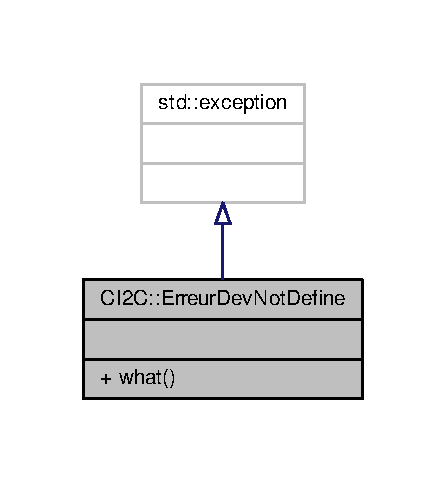
\includegraphics[width=214pt]{classCI2C_1_1ErreurDevNotDefine__inherit__graph}
\end{center}
\end{figure}


Graphe de collaboration de C\+I2\+C\+:\+:Erreur\+Dev\+Not\+Define\+:
\nopagebreak
\begin{figure}[H]
\begin{center}
\leavevmode
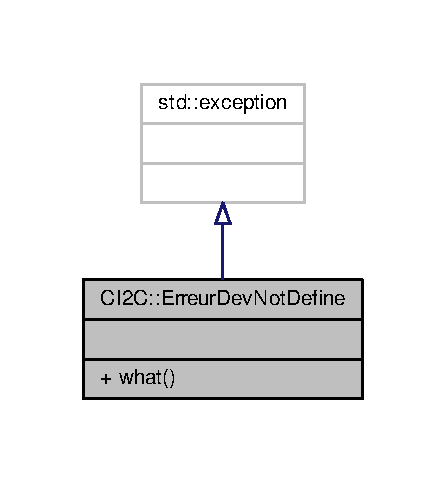
\includegraphics[width=214pt]{classCI2C_1_1ErreurDevNotDefine__coll__graph}
\end{center}
\end{figure}
\subsection*{Fonctions membres publiques}
\begin{DoxyCompactItemize}
\item 
\hypertarget{classCI2C_1_1ErreurDevNotDefine_a8c2f805ea7adc632db53c58437c2884e}{virtual const char $\ast$ {\bfseries what} () const noexcept}\label{classCI2C_1_1ErreurDevNotDefine_a8c2f805ea7adc632db53c58437c2884e}

\end{DoxyCompactItemize}


La documentation de cette classe a été générée à partir du fichier suivant \+:\begin{DoxyCompactItemize}
\item 
/home/jam/\+Bureau/\+C++/\+Classes/\+C\+R\+T\+C/\+C\+I2\+C/\hyperlink{CI2C_8h}{C\+I2\+C.\+h}\end{DoxyCompactItemize}

\hypertarget{classCI2C_1_1ErreurOpenDev}{\section{Référence de la classe C\+I2\+C\+:\+:Erreur\+Open\+Dev}
\label{classCI2C_1_1ErreurOpenDev}\index{C\+I2\+C\+::\+Erreur\+Open\+Dev@{C\+I2\+C\+::\+Erreur\+Open\+Dev}}
}


Graphe d'héritage de C\+I2\+C\+:\+:Erreur\+Open\+Dev\+:
\nopagebreak
\begin{figure}[H]
\begin{center}
\leavevmode
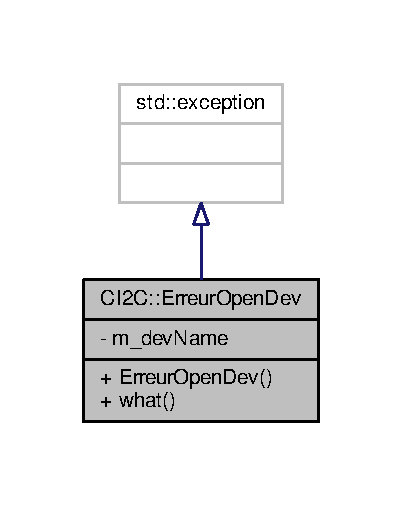
\includegraphics[width=193pt]{classCI2C_1_1ErreurOpenDev__inherit__graph}
\end{center}
\end{figure}


Graphe de collaboration de C\+I2\+C\+:\+:Erreur\+Open\+Dev\+:
\nopagebreak
\begin{figure}[H]
\begin{center}
\leavevmode
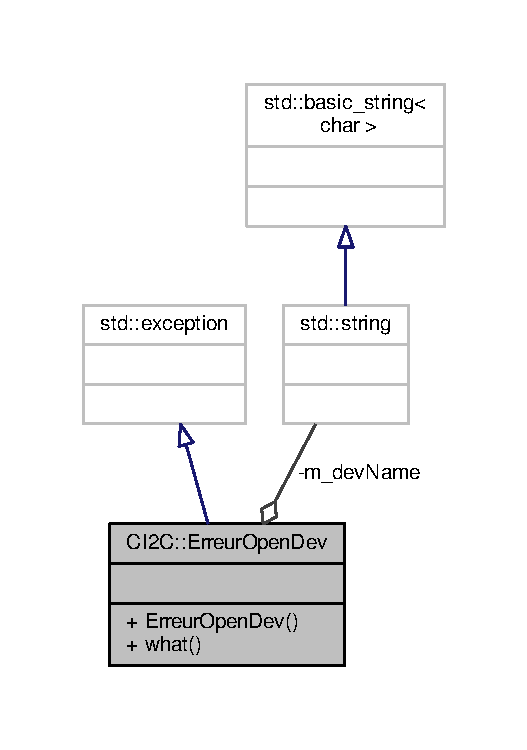
\includegraphics[width=253pt]{classCI2C_1_1ErreurOpenDev__coll__graph}
\end{center}
\end{figure}
\subsection*{Fonctions membres publiques}
\begin{DoxyCompactItemize}
\item 
\hypertarget{classCI2C_1_1ErreurOpenDev_ac741480179a06b9d23f4c5c49500a5e1}{{\bfseries Erreur\+Open\+Dev} (string dev\+Name)}\label{classCI2C_1_1ErreurOpenDev_ac741480179a06b9d23f4c5c49500a5e1}

\item 
\hypertarget{classCI2C_1_1ErreurOpenDev_a52441e7b0de2a74dd51c67504bb93fe1}{virtual const char $\ast$ {\bfseries what} () const noexcept}\label{classCI2C_1_1ErreurOpenDev_a52441e7b0de2a74dd51c67504bb93fe1}

\end{DoxyCompactItemize}
\subsection*{Attributs privés}
\begin{DoxyCompactItemize}
\item 
\hypertarget{classCI2C_1_1ErreurOpenDev_a19fcf1034384789940c900e32953e857}{string {\bfseries m\+\_\+dev\+Name}}\label{classCI2C_1_1ErreurOpenDev_a19fcf1034384789940c900e32953e857}

\end{DoxyCompactItemize}


La documentation de cette classe a été générée à partir du fichier suivant \+:\begin{DoxyCompactItemize}
\item 
/home/jam/\+Bureau/\+C++/\+Classes/\+C\+R\+T\+C/\+C\+I2\+C/\hyperlink{CI2C_8h}{C\+I2\+C.\+h}\end{DoxyCompactItemize}

\hypertarget{classCI2C_1_1ErreurRead}{\section{Référence de la classe C\+I2\+C\+:\+:Erreur\+Read}
\label{classCI2C_1_1ErreurRead}\index{C\+I2\+C\+::\+Erreur\+Read@{C\+I2\+C\+::\+Erreur\+Read}}
}


Graphe d'héritage de C\+I2\+C\+:\+:Erreur\+Read\+:
\nopagebreak
\begin{figure}[H]
\begin{center}
\leavevmode
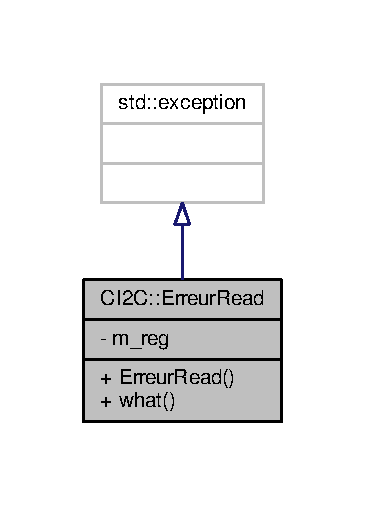
\includegraphics[width=175pt]{classCI2C_1_1ErreurRead__inherit__graph}
\end{center}
\end{figure}


Graphe de collaboration de C\+I2\+C\+:\+:Erreur\+Read\+:
\nopagebreak
\begin{figure}[H]
\begin{center}
\leavevmode
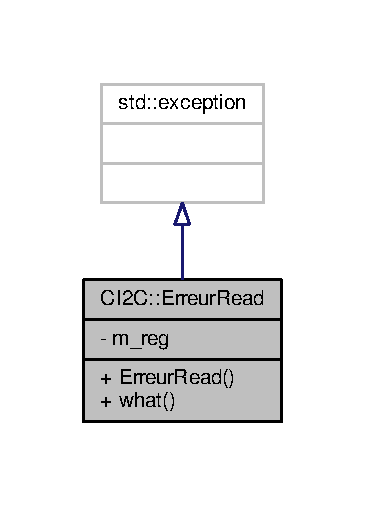
\includegraphics[width=175pt]{classCI2C_1_1ErreurRead__coll__graph}
\end{center}
\end{figure}
\subsection*{Fonctions membres publiques}
\begin{DoxyCompactItemize}
\item 
\hypertarget{classCI2C_1_1ErreurRead_a2006046ac1989f7d8f36e73365a7430d}{{\bfseries Erreur\+Read} (int reg)}\label{classCI2C_1_1ErreurRead_a2006046ac1989f7d8f36e73365a7430d}

\item 
\hypertarget{classCI2C_1_1ErreurRead_a43289e1f3f662de4ee81036a98b2ed55}{virtual const char $\ast$ {\bfseries what} () const noexcept}\label{classCI2C_1_1ErreurRead_a43289e1f3f662de4ee81036a98b2ed55}

\end{DoxyCompactItemize}
\subsection*{Attributs privés}
\begin{DoxyCompactItemize}
\item 
\hypertarget{classCI2C_1_1ErreurRead_a8af2c5a4b9b952aa97537fd2c59745a5}{int {\bfseries m\+\_\+reg}}\label{classCI2C_1_1ErreurRead_a8af2c5a4b9b952aa97537fd2c59745a5}

\end{DoxyCompactItemize}


La documentation de cette classe a été générée à partir du fichier suivant \+:\begin{DoxyCompactItemize}
\item 
/home/jam/\+Bureau/\+C++/\+Classes/\+C\+R\+T\+C/\+C\+I2\+C/\hyperlink{CI2C_8h}{C\+I2\+C.\+h}\end{DoxyCompactItemize}

\hypertarget{classCI2C_1_1ErreurSetAddrSlave}{\section{Référence de la classe C\+I2\+C\+:\+:Erreur\+Set\+Addr\+Slave}
\label{classCI2C_1_1ErreurSetAddrSlave}\index{C\+I2\+C\+::\+Erreur\+Set\+Addr\+Slave@{C\+I2\+C\+::\+Erreur\+Set\+Addr\+Slave}}
}


Graphe d'héritage de C\+I2\+C\+:\+:Erreur\+Set\+Addr\+Slave\+:
\nopagebreak
\begin{figure}[H]
\begin{center}
\leavevmode
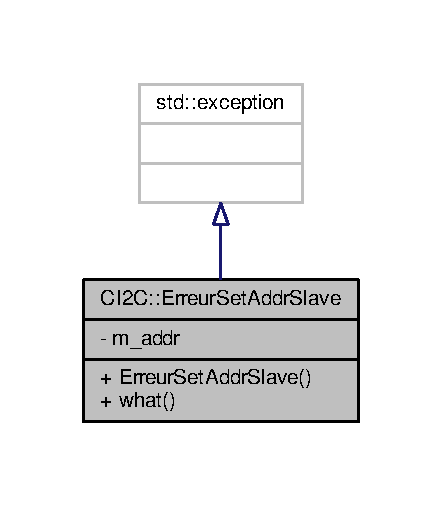
\includegraphics[width=212pt]{classCI2C_1_1ErreurSetAddrSlave__inherit__graph}
\end{center}
\end{figure}


Graphe de collaboration de C\+I2\+C\+:\+:Erreur\+Set\+Addr\+Slave\+:
\nopagebreak
\begin{figure}[H]
\begin{center}
\leavevmode
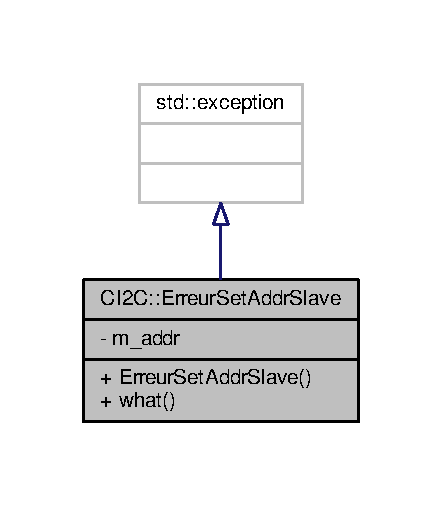
\includegraphics[width=212pt]{classCI2C_1_1ErreurSetAddrSlave__coll__graph}
\end{center}
\end{figure}
\subsection*{Fonctions membres publiques}
\begin{DoxyCompactItemize}
\item 
\hypertarget{classCI2C_1_1ErreurSetAddrSlave_ac92f34eb7c68e1b29ae55e0b147bdc02}{{\bfseries Erreur\+Set\+Addr\+Slave} (int addr)}\label{classCI2C_1_1ErreurSetAddrSlave_ac92f34eb7c68e1b29ae55e0b147bdc02}

\item 
\hypertarget{classCI2C_1_1ErreurSetAddrSlave_a6f82e7fa42f2ea5bb39d9c06517c5b09}{virtual const char $\ast$ {\bfseries what} () const noexcept}\label{classCI2C_1_1ErreurSetAddrSlave_a6f82e7fa42f2ea5bb39d9c06517c5b09}

\end{DoxyCompactItemize}
\subsection*{Attributs privés}
\begin{DoxyCompactItemize}
\item 
\hypertarget{classCI2C_1_1ErreurSetAddrSlave_aebf96cc2020fd45215280d41648151d8}{int {\bfseries m\+\_\+addr}}\label{classCI2C_1_1ErreurSetAddrSlave_aebf96cc2020fd45215280d41648151d8}

\end{DoxyCompactItemize}


La documentation de cette classe a été générée à partir du fichier suivant \+:\begin{DoxyCompactItemize}
\item 
/home/jam/\+Bureau/\+C++/\+Classes/\+C\+R\+T\+C/\+C\+I2\+C/\hyperlink{CI2C_8h}{C\+I2\+C.\+h}\end{DoxyCompactItemize}

\hypertarget{classCI2C_1_1ErreurSlaveNotDefine}{\section{Référence de la classe C\+I2\+C\+:\+:Erreur\+Slave\+Not\+Define}
\label{classCI2C_1_1ErreurSlaveNotDefine}\index{C\+I2\+C\+::\+Erreur\+Slave\+Not\+Define@{C\+I2\+C\+::\+Erreur\+Slave\+Not\+Define}}
}


Graphe d'héritage de C\+I2\+C\+:\+:Erreur\+Slave\+Not\+Define\+:
\nopagebreak
\begin{figure}[H]
\begin{center}
\leavevmode
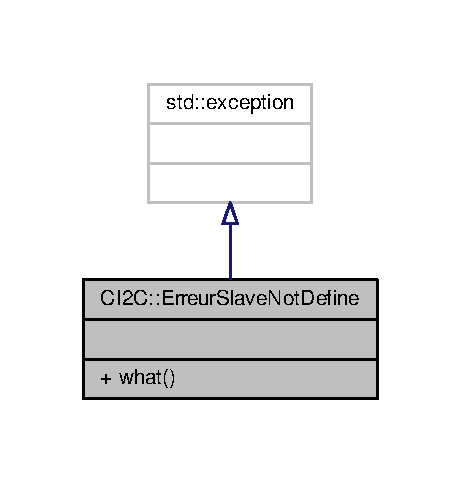
\includegraphics[width=221pt]{classCI2C_1_1ErreurSlaveNotDefine__inherit__graph}
\end{center}
\end{figure}


Graphe de collaboration de C\+I2\+C\+:\+:Erreur\+Slave\+Not\+Define\+:
\nopagebreak
\begin{figure}[H]
\begin{center}
\leavevmode
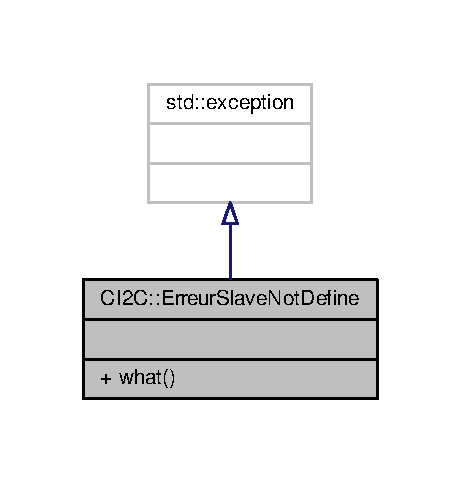
\includegraphics[width=221pt]{classCI2C_1_1ErreurSlaveNotDefine__coll__graph}
\end{center}
\end{figure}
\subsection*{Fonctions membres publiques}
\begin{DoxyCompactItemize}
\item 
\hypertarget{classCI2C_1_1ErreurSlaveNotDefine_a7efd5525f6598a091e21519cfcc3cd95}{virtual const char $\ast$ {\bfseries what} () const noexcept}\label{classCI2C_1_1ErreurSlaveNotDefine_a7efd5525f6598a091e21519cfcc3cd95}

\end{DoxyCompactItemize}


La documentation de cette classe a été générée à partir du fichier suivant \+:\begin{DoxyCompactItemize}
\item 
/home/jam/\+Bureau/\+C++/\+Classes/\+C\+R\+T\+C/\+C\+I2\+C/\hyperlink{CI2C_8h}{C\+I2\+C.\+h}\end{DoxyCompactItemize}

\hypertarget{classCI2C_1_1ErreurWrite}{\section{Référence de la classe C\+I2\+C\+:\+:Erreur\+Write}
\label{classCI2C_1_1ErreurWrite}\index{C\+I2\+C\+::\+Erreur\+Write@{C\+I2\+C\+::\+Erreur\+Write}}
}


Graphe d'héritage de C\+I2\+C\+:\+:Erreur\+Write\+:
\nopagebreak
\begin{figure}[H]
\begin{center}
\leavevmode
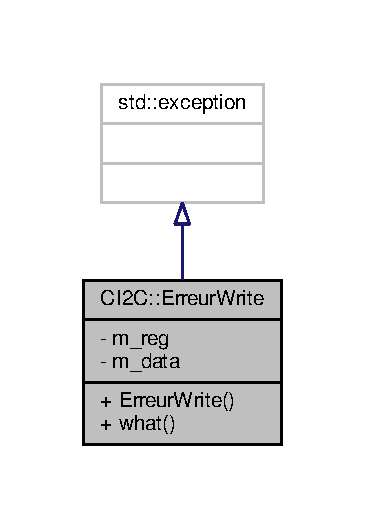
\includegraphics[width=175pt]{classCI2C_1_1ErreurWrite__inherit__graph}
\end{center}
\end{figure}


Graphe de collaboration de C\+I2\+C\+:\+:Erreur\+Write\+:
\nopagebreak
\begin{figure}[H]
\begin{center}
\leavevmode
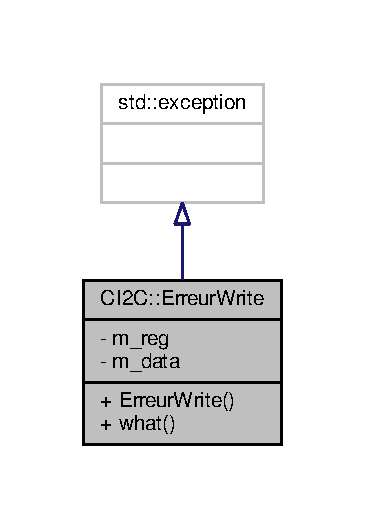
\includegraphics[width=175pt]{classCI2C_1_1ErreurWrite__coll__graph}
\end{center}
\end{figure}
\subsection*{Fonctions membres publiques}
\begin{DoxyCompactItemize}
\item 
\hypertarget{classCI2C_1_1ErreurWrite_a8d3b2f6b46d6bb5e4b26e5fdce8e80b4}{{\bfseries Erreur\+Write} (int reg, int data)}\label{classCI2C_1_1ErreurWrite_a8d3b2f6b46d6bb5e4b26e5fdce8e80b4}

\item 
\hypertarget{classCI2C_1_1ErreurWrite_ad76aa069d233146923c4a244d2da9665}{virtual const char $\ast$ {\bfseries what} () const noexcept}\label{classCI2C_1_1ErreurWrite_ad76aa069d233146923c4a244d2da9665}

\end{DoxyCompactItemize}
\subsection*{Attributs privés}
\begin{DoxyCompactItemize}
\item 
\hypertarget{classCI2C_1_1ErreurWrite_a0271678b0343dd18ad8113ab3dd579d2}{int {\bfseries m\+\_\+reg}}\label{classCI2C_1_1ErreurWrite_a0271678b0343dd18ad8113ab3dd579d2}

\item 
\hypertarget{classCI2C_1_1ErreurWrite_a3ba1d239d00892177274b494e987862b}{int {\bfseries m\+\_\+data}}\label{classCI2C_1_1ErreurWrite_a3ba1d239d00892177274b494e987862b}

\end{DoxyCompactItemize}


La documentation de cette classe a été générée à partir du fichier suivant \+:\begin{DoxyCompactItemize}
\item 
/home/jam/\+Bureau/\+C++/\+Classes/\+C\+R\+T\+C/\+C\+I2\+C/\hyperlink{CI2C_8h}{C\+I2\+C.\+h}\end{DoxyCompactItemize}

\chapter{Documentation des fichiers}
\hypertarget{CI2C_8cpp}{\section{Référence du fichier /home/jam/\+Bureau/\+C++/\+Classes/\+C\+R\+T\+C/\+C\+I2\+C/\+C\+I2\+C.cpp}
\label{CI2C_8cpp}\index{/home/jam/\+Bureau/\+C++/\+Classes/\+C\+R\+T\+C/\+C\+I2\+C/\+C\+I2\+C.\+cpp@{/home/jam/\+Bureau/\+C++/\+Classes/\+C\+R\+T\+C/\+C\+I2\+C/\+C\+I2\+C.\+cpp}}
}


Contient la définition de la classe \hyperlink{classCI2C}{C\+I2\+C}.  


{\ttfamily \#include \char`\"{}C\+I2\+C.\+h\char`\"{}}\\*
Graphe des dépendances par inclusion de C\+I2\+C.\+cpp\+:
\nopagebreak
\begin{figure}[H]
\begin{center}
\leavevmode
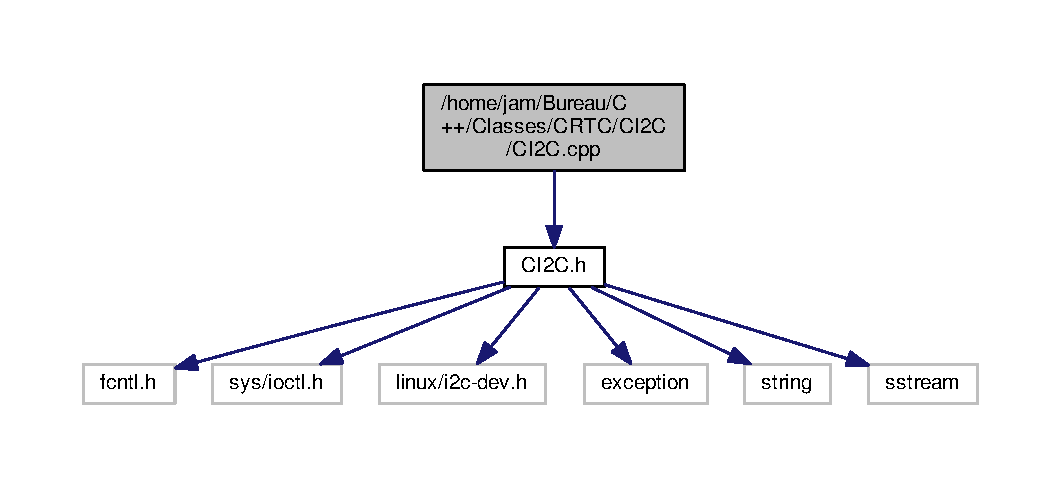
\includegraphics[width=350pt]{CI2C_8cpp__incl}
\end{center}
\end{figure}


\subsection{Description détaillée}
Contient la définition de la classe \hyperlink{classCI2C}{C\+I2\+C}. 


\hypertarget{CI2C_8h}{\section{Référence du fichier /home/jam/\+Bureau/\+C++/\+Classes/\+C\+R\+T\+C/\+C\+I2\+C/\+C\+I2\+C.h}
\label{CI2C_8h}\index{/home/jam/\+Bureau/\+C++/\+Classes/\+C\+R\+T\+C/\+C\+I2\+C/\+C\+I2\+C.\+h@{/home/jam/\+Bureau/\+C++/\+Classes/\+C\+R\+T\+C/\+C\+I2\+C/\+C\+I2\+C.\+h}}
}


Contient la declaration de la \hyperlink{classCI2C}{C\+I2\+C}.  


{\ttfamily \#include $<$fcntl.\+h$>$}\\*
{\ttfamily \#include $<$sys/ioctl.\+h$>$}\\*
{\ttfamily \#include $<$linux/i2c-\/dev.\+h$>$}\\*
{\ttfamily \#include $<$exception$>$}\\*
{\ttfamily \#include $<$string$>$}\\*
{\ttfamily \#include $<$sstream$>$}\\*
Graphe des dépendances par inclusion de C\+I2\+C.\+h\+:
\nopagebreak
\begin{figure}[H]
\begin{center}
\leavevmode
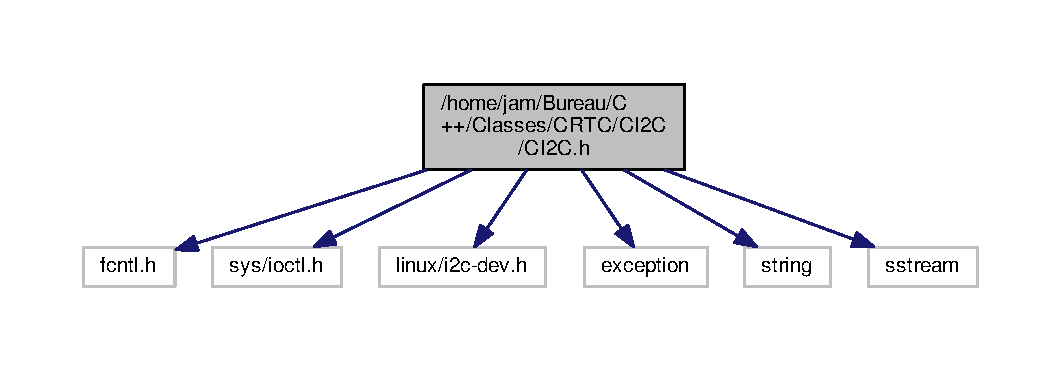
\includegraphics[width=350pt]{CI2C_8h__incl}
\end{center}
\end{figure}
Ce graphe montre quels fichiers incluent directement ou indirectement ce fichier \+:
\nopagebreak
\begin{figure}[H]
\begin{center}
\leavevmode
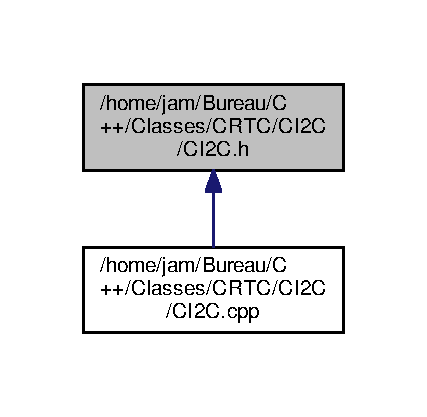
\includegraphics[width=205pt]{CI2C_8h__dep__incl}
\end{center}
\end{figure}
\subsection*{Classes}
\begin{DoxyCompactItemize}
\item 
class \hyperlink{classCI2C}{C\+I2\+C}
\begin{DoxyCompactList}\small\item\em Cette classe \hyperlink{classCI2C}{C\+I2\+C} permet de lire/écrire les valeurs de registres des esclaves d'un bus I2\+C. \end{DoxyCompactList}\item 
class \hyperlink{classCI2C_1_1ErreurWrite}{C\+I2\+C\+::\+Erreur\+Write}
\item 
class \hyperlink{classCI2C_1_1ErreurRead}{C\+I2\+C\+::\+Erreur\+Read}
\item 
class \hyperlink{classCI2C_1_1ErreurOpenDev}{C\+I2\+C\+::\+Erreur\+Open\+Dev}
\item 
class \hyperlink{classCI2C_1_1ErreurSetAddrSlave}{C\+I2\+C\+::\+Erreur\+Set\+Addr\+Slave}
\item 
class \hyperlink{classCI2C_1_1ErreurDevNotDefine}{C\+I2\+C\+::\+Erreur\+Dev\+Not\+Define}
\item 
class \hyperlink{classCI2C_1_1ErreurSlaveNotDefine}{C\+I2\+C\+::\+Erreur\+Slave\+Not\+Define}
\end{DoxyCompactItemize}


\subsection{Description détaillée}
Contient la declaration de la \hyperlink{classCI2C}{C\+I2\+C}. 


\hypertarget{CRTC_8h}{\section{Référence du fichier /home/jam/\+Bureau/\+C++/\+Classes/\+C\+R\+T\+C/\+C\+R\+T\+C.h}
\label{CRTC_8h}\index{/home/jam/\+Bureau/\+C++/\+Classes/\+C\+R\+T\+C/\+C\+R\+T\+C.\+h@{/home/jam/\+Bureau/\+C++/\+Classes/\+C\+R\+T\+C/\+C\+R\+T\+C.\+h}}
}


\subsection{Description détaillée}
Déclaration de la classe \hyperlink{classCRTC}{C\+R\+T\+C} 
%--- End generated contents ---

% Index
\newpage
\phantomsection
\addcontentsline{toc}{chapter}{Index}
\printindex

\end{document}
